\section{Implementation of a Rapport Agent}

\begin{figure*}
	\centering
	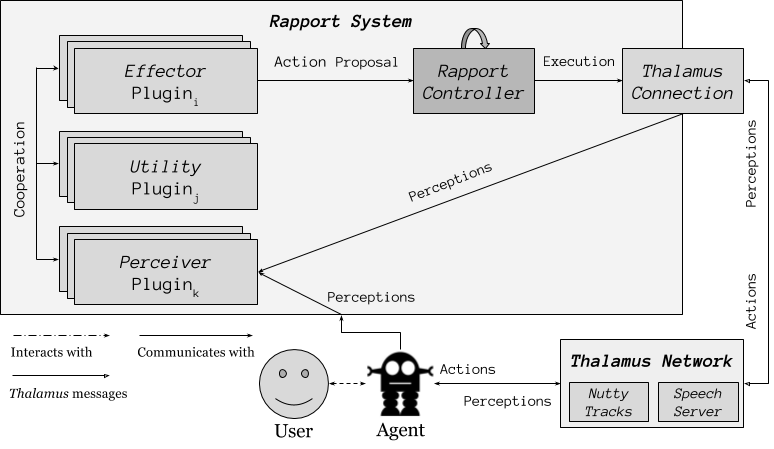
\includegraphics[width=0.6\textwidth]{RapportControllerArchitectureOverview.png}
	\caption{Depiction of the developed extension of \ac{SERA} to build rapport strategies on robotic agents.}
	\label{fig:rapport:archicture}
\end{figure*}

The system has the following goals:
\begin{enumerate}
	\item Support interruption of actions with custom strategies;
	\item Support replacement of actions using a prioritisation mechanism;
	\item Promote re-usage of interaction strategies on different \ac{HRI} scenarios.
\end{enumerate}

The system follows a plugin-based architecture that replaces \textit{Skene}. The communication is done through method calls, limiting the number of network messages. %Identical to \ac{SERA}, the project was developed in Visual Studio on Microsoft Window. 

Following Figure~\ref{fig:rapport:archicture}, the implemented architecture contains the following elements:
\begin{itemize}
	\item \textbf{\textit{Effector Plugins}}: proposes actions and enables/disables plugins;
	\item \textbf{\textit{Perceiver Plugins}}: perceives the external world and informs the interested plugins;
	\item \textbf{\textit{Utility Plugins}}: general purpose plugin that can be used to, for example, store interactional data;
	\item \textbf{\textit{Rapport Controller}}: manages the plugins and the proposed actions sent by the \textit{Effectors}. Conflicts may arise causing interruptions and/or replacement of actions;
	\item \textbf{\textit{Thalamus Connection}}: bridges the system with the \textit{Thalamus Network}, obtaining actions feedback (beginning and end), and provides connection to the \textit{Nutty Tracks} and \textit{Speech Server} to trigger animations or utterances, respectively.
\end{itemize}


Following the same Figure~\ref{fig:rapport:archicture}, there are five types of connections:
\begin{itemize}
	\item \textbf{Cooperation}: communication between plugins.
	\item \textbf{Perceptions}: perceptual information;
	\item \textbf{Action Proposal}: behaviour intentions sent by \textit{Effectors};
	\item \textbf{Execution}: set of actions triggered periodically by the 	
	\item \textit{Rapport Controller} - execution, interruptions or replacement;
	\item \textbf{Actions}: decisive messages that trigger animations or utterances;
\end{itemize}

%%%%%%%%%%%%%%%%%%%%%%%%%%%%%%%%%%%%%%%%%%%%%%%%%%%%%%%%%%%%%%%%%%%%%%%%%%%%%%%%%%%%%%%%%%%%%%%%%%
\subsection{Rapport Controller}
\label{sec:rapportController}

The main responsibilities of the \textit{Rapport Controller} are:
\begin{itemize}
	\item Load and manage the lifecycle of the plugins;
	\item Establish link between different plugins;
	\item Manage the proposed actions sent by the \textit{Effectors}.
\end{itemize}

\subsection{Plugins Lifecycle}
\label{sub:sec:pluginLifecycle}

At the startup, the \textit{Rapport Controller} loads the available plugins from a pre-defined folder. They are all enabled by default, unless specified otherwise through a configuration file. During this stage, following Figure~\ref{fig:pluginLifecycle}, each plugin follows a two-step initialisation:
\begin{enumerate}
	\item \textbf{Initialisation}: initialise internal variables;
	\item \textbf{Retrieve Dependencies}: retrieve plugins that it depends on (e.g., \textit{Effectors} typically requires \textit{Perceivers}).
\end{enumerate}

After initialisation, if the controller is running, \textit{Perceivers} capture external world stimuli and notify the interested \textit{Effectors} which will attempt to modify the agent's behaviour concurrently by proposing actions to the \textit{Rapport Controller}. 

\begin{figure}[H]
	\centering
	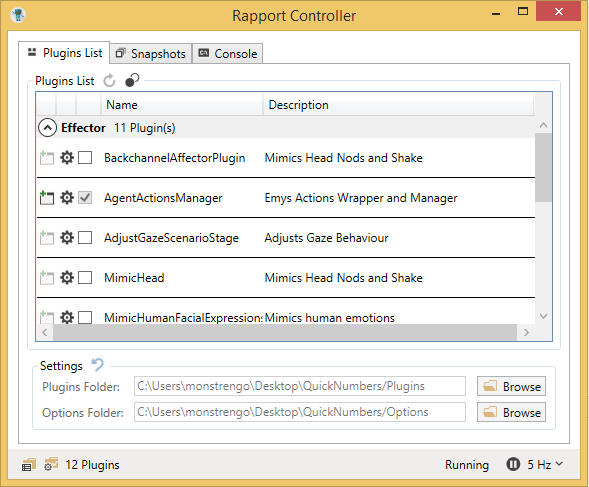
\includegraphics[width=0.4\textwidth]{PluginsList.png}
	\caption{\ac{GUI} representation of the system.}
	\label{fig:pluginList}
\end{figure}

After initialisation, the plugins can be either running or paused depending on the state of the controller itself. The plugins may be disabled and re-enabled in runtime, either through the \ac{GUI} (Figure~\ref{fig:pluginList}) or automatically by \textit{Effectors}. They are automatically deactivated and disposed whenever there is an error in any of the state transitions.

\begin{figure}[H]
	\centering
	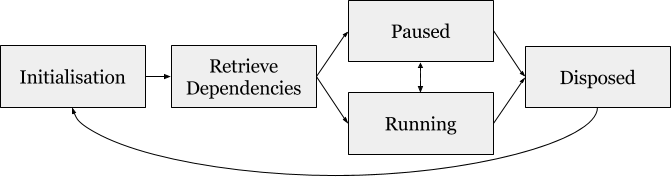
\includegraphics[width=0.45\textwidth]{PluginsLifecycle.png}
	\caption{Plugin's lifecycle.}
	\label{fig:pluginLifecycle}
\end{figure}

\subsection{Managing Actions}
\label{sub:sec:managingActions}

The \textit{Rapport Controller} periodically captures a snapshot of the agent's pending and current action proposals sent by the \textit{Effectors}. Each snapshot contains the timestamp and the list of the actions that the controller is tracking at a given instance (Figure~\ref{fig:controllerSnapshots}). Each action contains:
\begin{itemize}
	\item Priority - in relation with others;
	\item \textit{Group} - Portion of the body it is trying to manipulate;
	\item Execution description - anonymous function to customise the behaviour;
	\item Interruption description - anonymous function to customise the behaviour;
	\item Status - \textit{pending}, \textit{executing}, \textit{executed} or \textit{interrupted};
	\item Starting time;
	\item Timeout - maximum executing duration of the action;
	\item \textit{Thalamus} identifier - to monitor when actions have finished.
\end{itemize}

\begin{figure}[H]
	\centering
	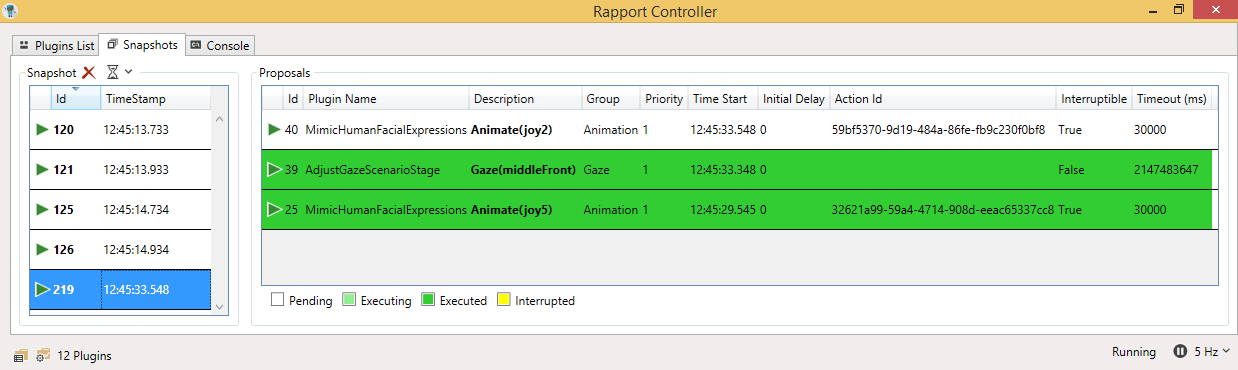
\includegraphics[width=0.47\textwidth]{ScreenshotSnapshots.png}
	\caption{Graphical representation of the snapshots captured periodically by the \textit{Rapport Controller}}
	\label{fig:controllerSnapshots}
\end{figure}

It should be noted that, to modify the agent's behaviour, the execution description (anonymous function) must at least contain the \textit{Thalamus} message that will make the agent act (\textit{Speech Server} or \textit{Nutty Tracks}).


As long as there is no action executing with the same \textit{Group}, there are no conflicts. If there is, as long as the action has not expired due to a timeout, the executing action with the lowest priority is interrupted (orange area in Figure~\ref{fig:conflict_interrupt}), and replaced. If the received proposal has lower priority than the current one in execution, then the former is ignored.

\begin{figure}[H]
	\centering
	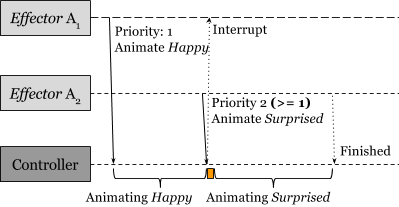
\includegraphics[width=0.4\textwidth]{ConflictingAndInterrupt.png}
	\caption{The action with higher priority, interrupts and replaces the action in execution.}
	\label{fig:conflict_interrupt}
\end{figure}


The priority is specified by the researcher, however, as a rule of thumb, idle actions should have a lower priority than actions that are triggered by discreet states. For example, a occasional smile should have lower priority than a backchannel behaviour that is triggered momentarily.

%%%%%%%%%%%%%%%%%%%%%%%%%%%%%%%%%%%%%%%%%%%%%%%%%%%%%%%%%%%%%%%%%%%%%%%%%%%%%%%%%%%%%%%%%%%%%%%%%%%%%%%%%%%%%%%%%%%%%%%%%%%%%%%%%%%%%%%%%%%%%%%%%%%%%%%%%%%%%%%%%%%%%%%%%%%%%%%%%%%%%%%%%%%%%%%%%%%%%%%%%%

\section{Plugins}
\label{sec:plugins}

There are three types of plugins: \textit{Effector}, \textit{Perceiver}, or \textit{Utility}. \textit{Effector} is the only type capable of proposing actions and changing the status of other plugins.

To promote reusability, researchers only need only to focus on the essentials components of the plugin as the system already provides the tools to handle, for example, optional \ac{GUI} and configuration files. The configuration file is a \ac{XML} document that is loaded during start-up and can be modified in runtime, by both technical and non-technical developers allowing tailoring the agent to different \ac{HRI} scenarios.

\begin{lstlisting}[caption={Excerpt of the configuration file used by Mimic Facial Expressions \textit{Effector}.}, label={lst:MimicFacialExpressionsSettings},language=XML]
<MimicFacialExpressionsSettings>
  <MinimumDelayMsBetweenActions>3500</MinimumDelayMsBetweenActions>
  <Happy>
    <TriggerProbability>0.48</TriggerProbability>
    <MinimumIntensity>0.65</MinimumIntensity>
    <Priority>1</Priority>
    <BaseAnimation>sadness</BaseAnimation>
  </Happy>
</MimicFacialExpressionsSettings>
\end{lstlisting}

\subsection{Encountered issues}
\label{sub:sec:effectorPlugin}

It was identified that the capability of deactivating and enabling plugins in runtime would be useful as it allows specific rapport strategies to take effect on discrete sections of the scenario, instead of adding additional complexity to the plugins. This management can be handled by a separate higher-level plugin that maps the agent's state to the list of enabled rapport strategies, leaving the essential to the \textit{Effector}.

We also noticed that some \textit{Effectors} frequently interrupt themselves repeatedly. To solve this issue, they may, transparently to the developer, track internally its proposed actions, and add delays between each sent action proposal (i.e., proposals are ignored internally until the delay has elapsed). The researcher can choose one of the following levels:

\begin{itemize}
	\item \textbf{Unrestricted}: the \textit{Effector} must explicitly manage its proposed actions;
	\item \textbf{One Action Globally}: the \textit{Effector} cannot interrupt itself unless with a proposal with higher priority;
	\item \textbf{One Action Per Group}: same as \textit{One Action Globally} but with granular to the \textit{Group}.
\end{itemize}

\subsection{Agent Actions Manager}
\label{sub:sec:agentActionsManager}

%Mencionar que é este o plugin que tem a Thalamus Connection para executar acções

Agent Actions Manager is a \textit{Utility} plugin with the following goals:
\begin{itemize}
	\item Monitor agent's actions and notify the \textit{Rapport Controller};
	\item Provide convenient wrappers for common action proposals;
	\item Provide non-technical researchers tools to change the agent's behaviour using the developed prioritisation mechanism, without worrying about implementation details.
\end{itemize}

\begin{figure}[H]
	\centering
	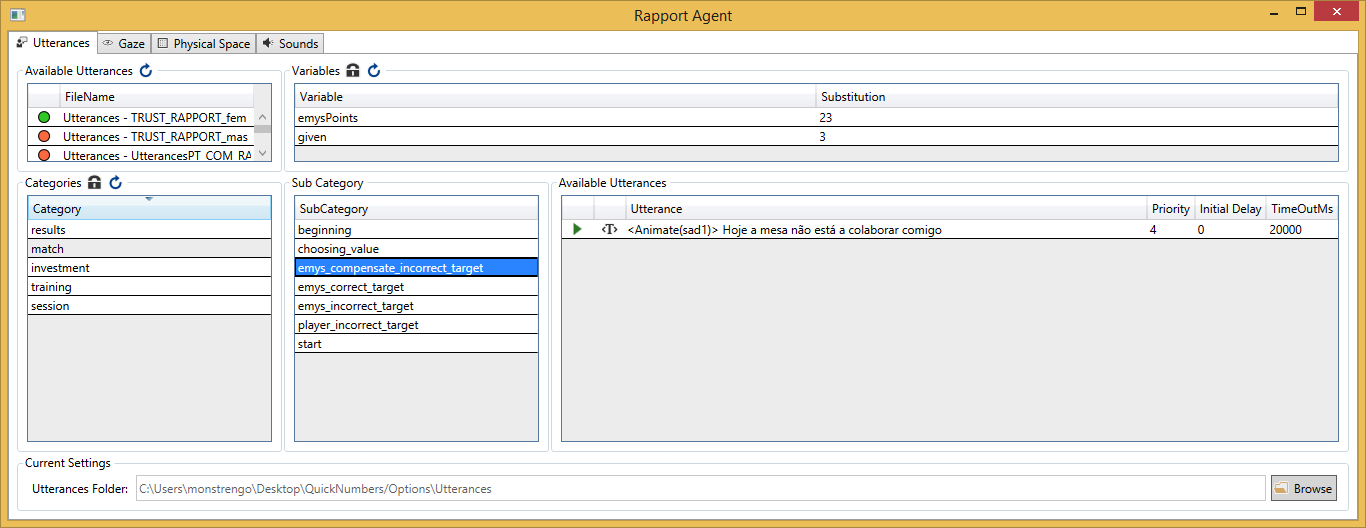
\includegraphics[width=0.45\textwidth]{ScreenshotAgentsManager.png}
	\caption{\ac{GUI} representation of the \textit{Utility} plugin Agent Action Manager.}
	\label{fig:agentActionsManagerScreenshot}
\end{figure}

The first objective is achieved by monitoring the messages that both \textit{Speech Server} and \textit{Nutty Tracks} send to the \textit{Thalamus Network}.

The last objective is an extension of \textit{Skene} using action proposals. The added behaviours may have additional arguments besides the required, as long as it follows the format specified in~\ref{eq:behaviour}. The additional arguments will default to the utterance priority, 0 and the utterance's timeout (see Figure~\ref{fig:extended:utterances}), respectively.

\begin{equation}
	<action(arg_1, arg_2, ..., arg_n, [priority],[delay],[timeout])>
	\label{eq:behaviour}
\end{equation}

The \textit{Effectors}, in order to take advantage of the Agent Action Manager's capabilities, they have to retrieve it in the \textit{Initialise dependencies} (Figure~\ref{fig:pluginLifecycle} in Section~\ref{sub:sec:pluginLifecycle}).

\begin{table*}[t]
	\centering
	\begin{tabular}{|l|l|l|l|l|l|}
	\hline
	\multicolumn{1}{|c|}{\textbf{Category}} & \multicolumn{1}{c|}{\textbf{Subcategory}} & \textbf{Utterance}                                                                                      & \textbf{Priority} & \textbf{Delay (ms)} & \textbf{Timeout (ms)} \\ \hline	
	intro & greet & \specialcell{Hi $|$\textit{Name}$|$! $<$gaze(person)$>$} & 2 & 0 & 30000 \\ \hline
	game & score & \specialcell{Yey! $<$Animate(surprise2, 3)$>$} & 2 & 0 & 30000 \\ \hline
	game & results & \specialcell{Managed $|$\texttt{Points}$|$!\\$<$gaze(person, 3, 500, 5000)$>$} & 2 & 0 & 30000 \\ \hline
	end & ending & \specialcell{I am glad to have met you!\\$<$animate(happy4, 4, 1000)$>$} & 3 & 0 & 30000 \\ \hline		
	\end{tabular}
	\caption{Example compilation of utterances compatible with the developed system.}
	\label{fig:extended:utterances}
\end{table*}


%%%%%%%%%%%%%%%%%%%%%%%%%%%%%%%%%%%%%%%%%%%%%%%%%%%%%%%%%%%%%%%%%%%%%%%%%%%%%%%%%%%%%%%%%%%%%%%%%%%%%%%%%%%%%%%%%%%%%%%%%%%%%%%%%%%%%%%%%%%%%%%%%%%%%%%%%%%%%%%%%%%%%%%%%%%%%%%%

\section{Rapport Strategies}


From the literature, we selected a representative set of successful rapport strategies that can be integrated with any \ac{SERA} agent, and implemented them as independent \textit{Effectors}.

\subsection{Supporting Technologies}


Following Figure~\ref{fig:SupportingTechnologiesOverview} there are four main softwares that supports the rapport strategies:
\begin{itemize}
	\item \textbf{\ac{SSI}}: recognise social signals in realtime~\footnote{\url{http://hcm-lab.de/projects/ssi/}} (prosody features and gestures)~\cite{Wagner2013};
	\item \textbf{SHORE}: recognise facial features from a video feed~\cite{Ruf2011};
	\item \textbf{GRETA\textsuperscript{PP}}: adapted version of GRETA to generate listener behaviour and redirect perceptions;
	\item \textbf{GRETA \textit{Perceiver} Plugin}: proxy between GRETA and the \textit{Rapport Controller}.
\end{itemize}

\begin{figure}[H]
	\centering
	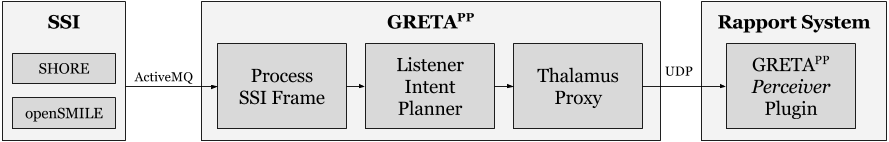
\includegraphics[width=0.45\textwidth]{figures/SupportingTechnologiesOverview.png}
	% TODO legenda
	\caption{Supporting technologies that supports the developed rapport strategies.}
	\label{fig:SupportingTechnologiesOverview}
\end{figure}

GRETA\textsuperscript{PP}, the main component, is a variation of the GRETA system~\cite{Niewiadomski2009} that contains solely its \textit{Listener Intention Planner} rule-based component. It additionally perceives head gestures and facial expressions using Kinect sensors and the video feed, respectively. The perceptions and the generated behaviour are sent to the GRETA \textit{Perceiver} Plugin using \ac{UDP} sockets so that it notifies the interested \textit{Effectors}. The system has a slight delay ($<$ 1 second), as the refresh rate default rate had to be halved to 5Hz so that the system could handle the resource heavy \ac{SSI}.

%%%%%%%%%%%%%%%%%%%%%%%%%%%%%%%%%%%%%%%%%%%%%%%%%%%%%%%%%%%%%%%%%%%%%%%%%%%%%%%%%%%%%%%%%%%%

\subsection{Facial Expression Mimicry}

The Facial Expression Mimicry \textit{Effector} mirrors SHORE's perceived emotion, mirroring human's unconscious reactions to emotions~\cite{Dimberg2000}. Given that emotions are continuous signals, the mimicry behaviours are triggered periodically according to empirical chosen probability values (Listing~\ref{lst:MimicFacialExpressionsSettings}). Nonetheless, the implementation of this plugin is not without issues as SHORE was detecting happy emotions in absence of faces. We solved that issue by applying a smoothing signal at the cost of increasing the delay from less than 1 second, to at most 3 seconds. In the end, we opted to remove the smoothing filter and compensate with disabling the \textit{Effector} when the user was not present.

\subsection{Head Gestures Mimicry}

Head Nod Mimicry \textit{Effector} focus on enhancing coordination mimicking head nods and head shakes~\cite{Riek2009, Andrist2014, Cassell2007, Wang2009}. The head gestures parameters (\texttt{intensity}, \texttt{repetitions} and \texttt{frequency}) are randomised in each action proposal following Listing~\ref{lst:headMimicSettings}, which makes the agent less robotic as its movement is not as repetitive as if were reusing the parameters.

\begin{lstlisting}[caption={Head Gestures Mimicry \textit{Effector} configuration file.},label={lst:headMimicSettings},language=XML]
<MimicHeadSettings>
  <MinimumDelayMsBetweenActions>2500</MinimumDelayMsBetweenActions>
  <Nod>
    <Priority>1</Priority>
    <MinimumIntensity>5</MinimumIntensity>
    <MaximumIntensity>10</MaximumIntensity>
    <MinimumRepetitions>2</MinimumRepetitions>
    <MaximumRepetitions>2</MaximumRepetitions>
    <MinimumFrequency>125</MinimumFrequency>
    <MaximumFrequency>160</MaximumFrequency>
    <TriggerProbability>1</TriggerProbability>
  </Nod>
</MimicHeadSettings>
\end{lstlisting}

\subsection{Mutual-Gaze}
The Mutual-Gaze \textit{Effector} focus on building rapport by enhancing mutual-attention following the work developed by Andrist et. al.~\cite{Andrist2015}. In short, the agent will swap between looking at the eyes of the participant and the game for pre-determined periods according to game stage and the person's personality. However, in this experiment, as we do not know the participant's personality we will assume that he is extrovert - Table~\ref{table:gazetimes}.

\begin{table}[H]
	\centering
	\begin{tabular}{|l|l|l|l|}
	\hline
	\multicolumn{1}{|c|}{\textbf{Personality}} & \multicolumn{2}{c|}{\textbf{Extrovert}}  \\ \hline
	\textbf{Phase}                             & \textbf{In-Task} & \textbf{Between-Task} \\ \hline
	Partner                                    & 2.66 (0.80)      & 3.91 (1.22)           \\ \hline
	Puzzle                                     & 4.04 (2.12)      & 1.01 (1.26)           \\ \hline
	\end{tabular}
	
	\caption{Means and standard deviations of gaze duration (in seconds) to the partner, and to the puzzle assuming extrovert personality. Adapted~\cite{Andrist2015}}.
	\label{table:gazetimes}
\end{table}

\subsection{Backchannel}
The Backchannel \textit{Effector} is based on the GRETA system that analyses variations of the pitch during the interaction to produce listener behaviour~\cite{Niewiadomski2009}. Presently, the \textit{Effector} only triggers head nods as we are  not capable of producing a convincing \textit{Hmm hmmm} with similar pitch as the generated voice by the \textit{Speech Server}.

However, we were unable to reduce the impact of noise (agent's robotic movement and voice) on the \ac{SSI} sensors, leading to excessive false positives. Despite the attempts of counteracting the issue through noise-suppressing directional microphone and adjusting sensors parameters, the issue persisted, therefore the Backchannel \textit{Effector} was not used during the studies.

%, and on the work developed by Huang et. al.~\ref{Buschmeier2011} on a virtual rapport agent. 
%Limited backchannel behaviours 

%Most of all, in order to build rapport more effectively, one should take into consideration if the above-mentioned strategies fit the study scenario, and if they are adequate to the person the agent is interacting with (e.g., introvert and extrovert people should be handled differently~\cite{Andrist2015}). This aspect is more relevant for enhancing positivity which is mostly built either through vocal interactions or through gestures. For this purpose, in order to build positivity, the developer must build their own \textit{Effector} or \textit{Effectors}.